% ============================================================
%  CHAPITRE 2 — Section 3 : Cadre d'évaluation & comparaison des EMS
% ============================================================

\section{Cadre d'évaluation \& comparaison des EMS}
\label{sec:simulation}

Les indicateurs définis dans les sections précédentes permettent de caractériser quantitativement la performance de toute EMS selon deux axes principaux~: la fiabilité d'alimentation à court terme (LPSP) et le coût de dégradation à long terme ($D_{\text{tot}}$). Il reste à définir le cadre dans lequel ces indicateurs sont calculés et exploités pour comparer les stratégies entre elles. Cette section décrit successivement la représentation graphique adoptée pour la comparaison des EMS (le plan de Pareto) et l'algorithme de simulation qui en permet le calcul. La troisième dimension de robustesse aux défaillances, sera traitée à la section~\ref{sec:robustesse}.

% ------------------------------------------------------------
\subsection{Représentation dans l'espace de performance (plan de Pareto)}
% ------------------------------------------------------------

À l'issue de chaque simulation, une EMS est entièrement caractérisée par le couple $(\mathrm{LPSP},\, D_{\text{tot}})$ qu'elle produit sur l'horizon de simulation. Il est alors naturel de représenter l'ensemble des EMS étudiées comme des points dans un espace de performance bidimensionnel, dont les axes correspondent respectivement à la LPSP (axe horizontal) et au coût de dégradation agrégé $D_{\text{tot}}$ exprimé en euros (axe vertical). Cette représentation constitue un plan de Pareto au sens large~: le point idéal, correspondant à une LPSP nulle et un coût de dégradation nul, se situe à l'origine, et toute amélioration sur un axe se fait en général au détriment de l'autre.

Cette visualisation présente plusieurs avantages pour la comparaison des EMS. D'une part, elle permet d'identifier immédiatement les stratégies dominées, c'est-à-dire celles pour lesquelles il existe une autre EMS offrant de meilleures performances sur les deux axes simultanément. D'autre part, elle met en évidence le front de Pareto, c'est-à-dire l'ensemble des EMS non dominées qui définissent la frontière des compromis réalisables~: toute amélioration d'un indicateur implique nécessairement une dégradation de l'autre. Enfin, cette représentation est particulièrement adaptée à la communication des résultats auprès des opérateurs ou des populations locales, à qui il appartient in fine de choisir le niveau de compromis acceptable entre confort d'alimentation et coût de maintenance.

Il est important de noter que certaines EMS peuvent ne pas être strictement dominées au sens de Pareto tout en étant peu attractives en pratique, par exemple si elles se trouvent très éloignées du front de compromis. L'interprétation de ce plan doit donc toujours s'accompagner d'une analyse du contexte applicatif et des priorités locales.

% ------------------------------------------------------------
\subsection{Algorithme de simulation}
% ------------------------------------------------------------

Le calcul des indicateurs de performance repose sur un algorithme de simulation en boucle fermée, dont le déroulement à l'intérieur d'un pas de temps est illustré à la Figure~\ref{fig:workflow}. À chaque pas de temps $t$, l'EMS établit une application de l'état instantané du système vers les consignes de contrôle. L'état instantané comprend le SoC de la batterie, le niveau d'hydrogène stocké $E_{\text{H2}}$, l'état de santé estimé des composants de stockage, ainsi que la demande de charge planifiée $\hat{P}_{\text{Load}}$ et la production PV $\hat{P}_{\text{PV}}$ à cet instant~; les consignes de contrôle sont les puissances des composants de stockage $\tilde{P}_{\text{bat}}(t)$, $\tilde{P}_{\text{FC}}(t)$ et $\tilde{P}_{\text{ELY}}(t)$.

Concrètement, l'EMS calcule d'abord la demande nette planifiée $\hat{P}_{\text{tot,plan}} = \hat{P}_{\text{Load}} - \hat{P}_{\text{PV}}$ puis, selon son signe (déficit ou surplus), applique un bloc de règles propre à la stratégie qui affecte la consigne du côté hydrogène, la batterie assurant le complément. Ce bloc de règles est générique~: n'importe laquelle des stratégies décrites à la section~\ref{sec:ems} peut y être insérée. Les consignes ainsi obtenues passent ensuite par un contrôle de faisabilité au regard des limites de fonctionnement~: puissances maximales des composants (actualisées par le SoH, cf.\ section~\ref{sec:soh}), bande de SoC admissible et capacité du réservoir d'hydrogène. Lorsque la commande demandée est infaisable, elle est saturée à ces limites. C'est précisément cette saturation qui peut créer une discordance entre la puissance planifiée et la puissance effectivement délivrée, et donc une perte d'alimentation contribuant à la LPSP. Une fois la commande faisable obtenue, les équations dynamiques régissant le comportement des composants sont résolues sur le pas de temps courant afin d'obtenir l'état du système au pas de temps suivant.

\begin{figure}[h!]
    \centering
    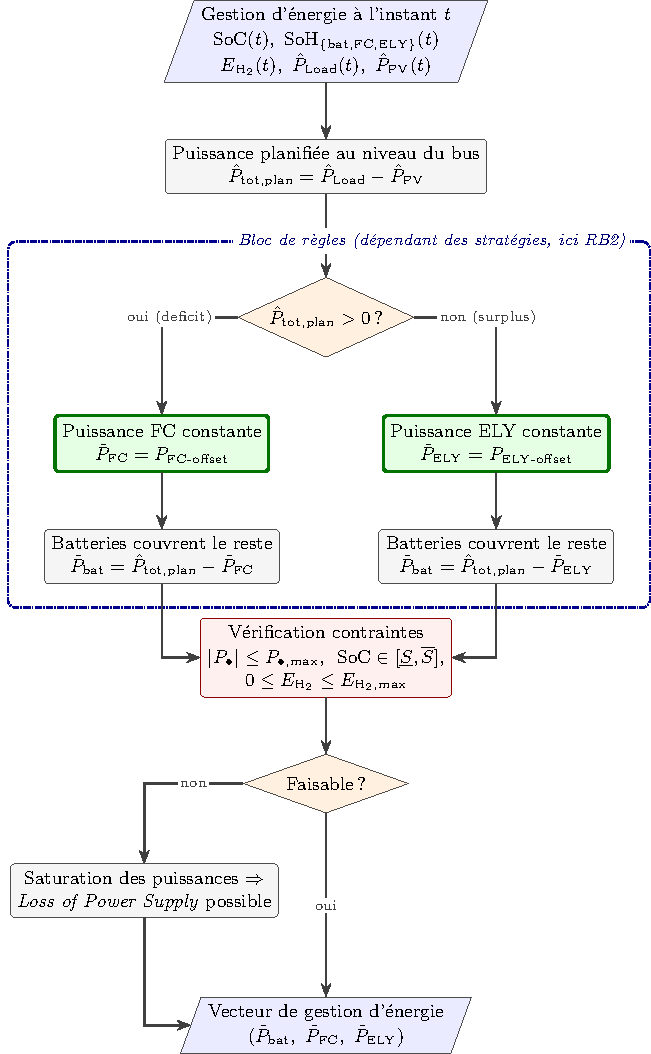
\includegraphics[width=.5\linewidth]{Chapitre 2/Simulation/Figures/workflow_ems_fr.pdf}
    \caption{Déroulé de la stratégie de gestion d'énergie sur un pas de temps $t$.}
    \label{fig:workflow}
\end{figure}
\FloatBarrier

Ce processus est répété sur l'intégralité de l'horizon de simulation, dont la durée est fixée à vingt-cinq ans. Ce choix permet d'observer clairement les processus de vieillissement à l'œuvre dans les composants de stockage, en incluant plusieurs remplacements de composants, tout en maintenant un temps de calcul raisonnable. Les simulations ont été implémentées en Python 3.12 et exécutées sur un poste de travail Intel Xeon W-2123 (4 cœurs, 3,60\,GHz, 32\,Go de RAM), avec un temps de calcul moyen d'environ dix minutes par simulation.

Le pas de temps de simulation est fixé à une heure. Seul le contrôle échantillonné à cette résolution est considéré dans ce travail~; le contrôle aux échelles de temps inférieures est supposé assuré par une couche de contrôle distincte. Les demandes de puissance à l'intérieur d'un intervalle d'une heure sont donc considérées comme constantes. Il convient toutefois de reconnaître que cette résolution temporelle peut conduire à une sous-estimation partielle des fluctuations de puissance infra-horaires, et par conséquent de certains phénomènes de dégradation survenant dans des conditions de fonctionnement plus rapides~\cite{e_toosi_impact_2023}\cite{pei_quick_2008}.

L'ensemble des simulations est réalisé dans les mêmes conditions environnementales et avec les mêmes modèles de composants, afin de garantir la comparabilité des résultats. Les profils de puissance PV et de demande de charge sont issus de données représentatives du microréseau résidentiel de La Réunion présenté au chapitre précédent. Il est par ailleurs supposé que l'estimation du SoH des composants est suffisamment précise pour que les plages de fonctionnement associées correspondent à la réalité.

À l'issue de la simulation, chaque EMS est représentée par un unique point dans le plan de Pareto décrit à la sous-section précédente. Ce cadre est appliqué à chaque stratégie considérée, permettant une comparaison directe et visuelle de l'ensemble des EMS étudiées. Ce cadre intègre par ailleurs, pour chaque stratégie, l'approche réactive au vieillissement décrite à la section~\ref{sec:soh}~: les plages de fonctionnement utilisées par le contrôle de faisabilité sont actualisées à chaque pas en fonction du SoH estimé des composants.